\documentclass[10pt,a4paper]{article}
% Compile with XeLaTeX for reliable French and English Unicode handling.
\usepackage[T1]{fontenc}
\usepackage{fontawesome5}
\usepackage[main=french,english]{babel}
\frenchsetup{StandardLists=true} % keep normal bullets, not French dashes

\usepackage[left=1.2cm,right=1.2cm,top=0.5cm,bottom=0.4cm]{geometry}
\usepackage{titlesec}
\usepackage{enumitem}
\usepackage[hidelinks]{hyperref}
\hypersetup{%
  pdftitle={Imane Taghzout — CV},
  pdfauthor={Imane Taghzout},
  pdfsubject={Data Scientist / Data Analyst / ML Engineer},
  pdfkeywords={Data Science, Machine Learning, LLM, RAG, Analytics, Power BI}
}
\usepackage{xcolor}
\usepackage{graphicx}
\usepackage{parskip}
\usepackage{setspace}
\usepackage{microtype}   % professional justification + character protrusion
\usepackage{tikz}

\definecolor{darkblue}{RGB}{30,60,110}
\definecolor{mutedgray}{RGB}{90,90,90}

\titleformat{\section}
  {\small\bfseries\color{darkblue}}
  {}{0em}{}
  [\vspace{-2pt}{\color{darkblue}\titlerule[0.4pt]}]
\titlespacing{\section}{0pt}{2pt}{2pt}
\setlist[itemize]{leftmargin=12pt, itemsep=0pt, topsep=0pt, partopsep=0pt, parsep=0pt}

\newcommand{\role}[3]{%
  \vspace{1pt}\noindent\textbf{#1} \textbar\ #2 \hfill \textcolor{mutedgray}{\small #3}\par\vspace{-2pt}
}

% -------------------- SHARED HEADER (tagline is the argument) --------------------
\newcommand{\cvheader}[1]{%
  \noindent
  \begin{minipage}[c]{0.76\textwidth}
      {\LARGE \textbf{IMANE TAGHZOUT}}\\[1pt]
      {\small #1}\\[3pt]
      {\footnotesize
      \textcolor{darkblue}{\faEnvelope}\ \href{mailto:taghzoutimane@gmail.com}{taghzoutimane@gmail.com} \quad
      \textcolor{darkblue}{\faPhone}\ +212 6 56 13 76 30 \quad
      \textcolor{darkblue}{\faMapMarker*}\ Casablanca, Morocco\\[1pt]
      \textcolor{darkblue}{\faLinkedin}\ \href{https://linkedin.com/in/imane-taghzout}{linkedin.com/in/imane-taghzout} \quad
      \textcolor{darkblue}{\faGithub}\ \href{https://github.com/imane-tag}{github.com/imane-tag} \quad
      \textcolor{darkblue}{\faGlobe}\ \href{https://imane-tag.github.io}{imane-tag.github.io}
      }
  \end{minipage}
  \hfill
  \begin{minipage}[c]{0.20\textwidth}
      \centering
      \IfFileExists{GEMMM.png}{%
          \begin{tikzpicture}
              \useasboundingbox (-1.15,-1.15) rectangle (1.15,1.15);
              \clip (0,0) circle (1.15cm);
              \node at (0,0) {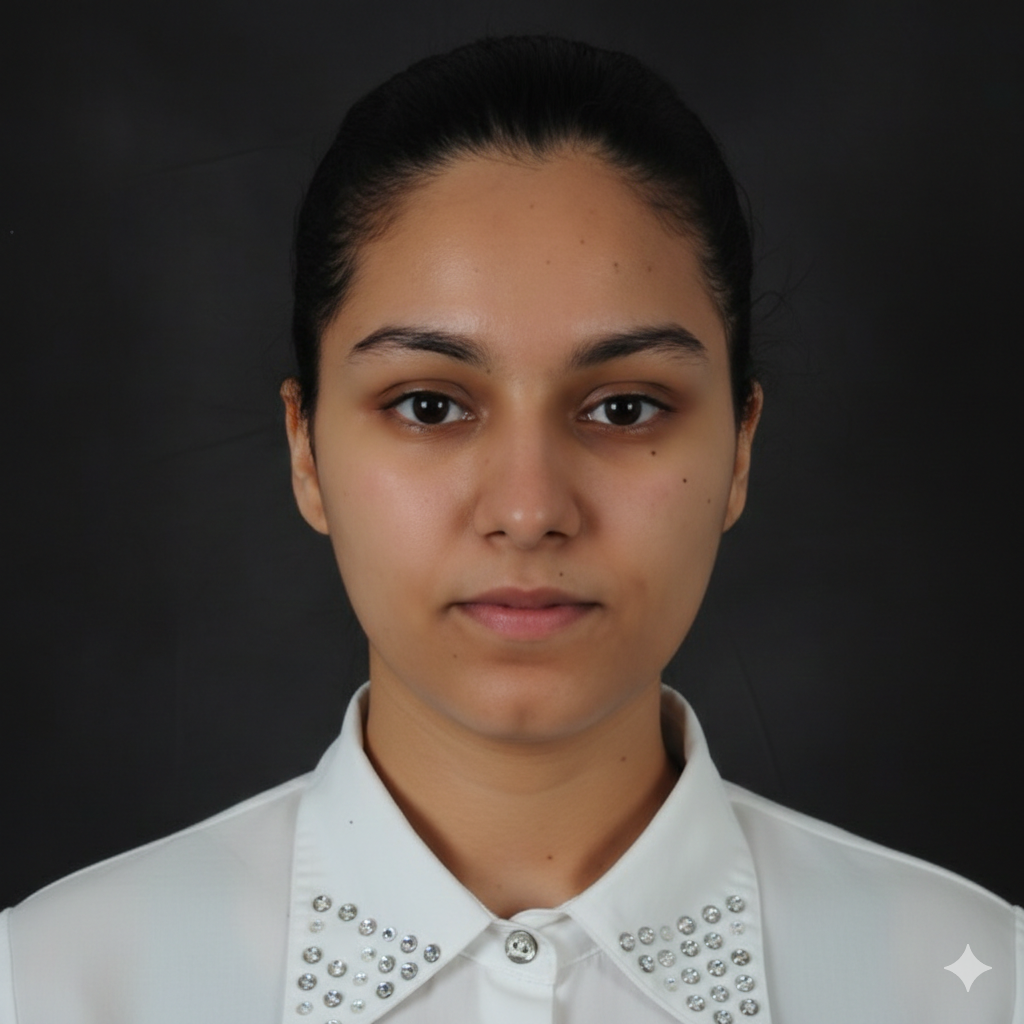
\includegraphics[width=2.3cm]{GEMMM.png}};
          \end{tikzpicture}
      }{%
          \begin{tikzpicture}
              \useasboundingbox (-1.15,-1.15) rectangle (1.15,1.15);
              \fill[darkblue!12] (0,0) circle (1.15cm);
              \draw[darkblue!45, line width=0.6pt] (0,0) circle (1.15cm);
              \node[darkblue, font=\Large\bfseries] at (0,0) {IT};
          \end{tikzpicture}
      }
  \end{minipage}
  \vspace{2pt}
}

\pagestyle{empty}
\begin{document}
\setstretch{0.83}
\renewcommand{\labelitemi}{\textbullet}

% =====================================================================
%  PAGE 1 — FRANÇAIS
% =====================================================================
\cvheader{\textcolor{darkblue}{\textbf{Data Scientist \& Data Analyst}} \textbar\ LLMs \textperiodcentered\ RAG \textperiodcentered\ ML appliqué \textperiodcentered\ Analytics \& BI}

\section*{PROFIL}
\small
Data Scientist (Master en Data Science \& IA, Mundiapolis University, Casablanca, 2025), avec \textbf{deux systèmes d'IA livrés de bout en bout} : un chatbot RAG multimodal chez Segula et un pipeline OCR + NLP chez Barid Al-Maghrib, ainsi qu'une contribution au développement d'une \textbf{plateforme de Generative Engine Optimization} chez Generovo. Allie ingénierie ML/LLM en production, analytics et décision fondée sur les données (SQL, Power BI, statistiques appliquées). Recherche de postes de \textbf{Data Scientist, Data Analyst ou Ingénieure ML} en IA appliquée, conseil en data \& IA, services financiers ou produits basés sur les LLM.

\section*{EXPÉRIENCE PROFESSIONNELLE}

\role{Generovo, startup studio IA}{Stagiaire Ingénieure IA Full-Stack}{Févr. 2026 \textbf{--} Juin 2026}
\begin{itemize}
    \item Contribution à la conception et au développement de \textbf{GEOCARA}, plateforme de bout en bout de \textbf{Generative Engine Optimization (GEO)} (audit $\to$ brief $\to$ rédaction $\to$ fact-checking $\to$ publication), conçue pour améliorer la visibilité de marque sur ChatGPT, Perplexity et Google AI Overviews.
    \item Conception et pilotage du \textbf{pipeline de contenu LLM} (prompts, sorties structurées validées par Zod, méthodologie de citation \og Answer First\fg{} de 40 à 80 mots) et du \textbf{fact-checking par IA}, avec publication bloquée sous un score de 70\,\%.
    \item Conception et développement de l'\textbf{Audit Engine} (Puppeteer + Cheerio), évaluant 6 métriques GEO sur 0\textbf{--}100 lors de crawls de 50 pages, ainsi que d'une \textbf{couche de suivi de visibilité} interrogeant plusieurs fournisseurs de LLM.
    \item Développement du \textbf{frontend web de GEOCARA} en \textbf{React + TypeScript} (Vite, Tailwind CSS), avec tableau de bord responsive pour visualiser les scores d'audit et la visibilité multi-moteurs.
\end{itemize}\vspace{-6pt}

\role{Segula Technologies, Casablanca}{Stagiaire AI \& Data Engineer}{Févr. 2025 \textbf{--} Juil. 2025}
\begin{itemize}
    \item Cadrage, développement et déploiement d'un \textbf{chatbot RAG d'entreprise multimodal} (SentenceTransformers + Qdrant + LLM) sur des milliers de pages de documentation interne ; réduction du temps moyen de recherche documentaire de $\approx$5\,min à $\approx$20\,s, libérant du temps d'ingénierie pour des tâches à plus forte valeur.
    \item Conception d'un \textbf{pipeline de recherche sémantique hybride} (BM25 + embeddings denses, reranking par cross-encoder), améliorant le Recall@5 de 0,61 à 0,81 sur un benchmark de 100 questions.
    \item Benchmark de 3 modèles d'embedding $\times$ 4 stratégies de chunking avec évaluation \textbf{LLM-as-judge} ; mise en production sur \textbf{FastAPI + Docker} avec logging structuré pour le suivi de dérive.
\end{itemize}\vspace{-6pt}

\role{Barid Al-Maghrib (BAM), Casablanca}{Stagiaire Data Science \& IA}{Mars 2024 \textbf{--} Juil. 2024}
\begin{itemize}
    \item Conception et déploiement d'un \textbf{pipeline de traitement documentaire OCR} (Python, OpenCV, Tesseract, post-traitement NLP), augmentant le débit de traitement de \textbf{30\,\%} par rapport au flux semi-manuel précédent.
    \item Développement et lancement d'une \textbf{application web} interne automatisant l'ingestion documentaire et l'extraction de données structurées, adoptée sur plusieurs flux.
    \item Amélioration de l'extraction via un \textbf{prétraitement tenant compte de la mise en page} et des règles post-OCR personnalisées, réduisant la relecture manuelle de \textbf{40\,\%}.
\end{itemize}\vspace{-6pt}

\role{Ministère de l'Énergie et des Mines, Casablanca}{Stagiaire Administration Systèmes \& Réseaux}{Avr. 2022 \textbf{--} Juil. 2022}
\begin{itemize}
    \item Administration d'\textbf{Active Directory} et d'une infrastructure virtualisée en cluster ; supervision des systèmes serveurs et réseaux ; mise en place de procédures de sauvegarde et de restauration pour soutenir disponibilité, performance et intégrité des données.
\end{itemize}

\section*{FORMATION}
\small
\textbf{2025} \textbar\ \textbf{Master en Data Science \& Intelligence Artificielle} — Université Mundiapolis, Casablanca, Maroc\\
\textbf{2024} \textbar\ \textbf{Programme Data Science} (16 mois) — ALX Africa, Casablanca, Maroc\\
\textbf{2023} \textbar\ \textbf{Formation Fondamentaux de la Cybersécurité} (6 mois) — Cyber4D\\
\textbf{2021} \textbar\ \textbf{Licence en Mathématiques \& Informatique} — Université Hassan II, Casablanca, Maroc

\section*{PROJETS}
\begin{itemize}
    \item \textbf{Prévision d'utilisation CPU} \textit{(ML de séries temporelles)} — ensemble SARIMAX + LightGBM ; backtest walk-forward sur 12 mois, MAPE $\approx$\textbf{8\,\%} contre $\approx$18\,\% pour une référence naïve saisonnière ; aide au dimensionnement des capacités d'infrastructure.
    \item \textbf{Analyse des prix immobiliers, Maroc} \textit{(Data Analytics)} — pipeline ETL collectant plus de 30\,000 annonces sur Avito, Sarouty et Mubawab ; analyse exploratoire et statistique identifiant les principaux déterminants de prix par ville et type de bien.
    \item \textbf{Prédiction du cours de l'or} \textit{(Deep Learning)} — modèles LSTM et GRU sur 10 ans de données historiques ; le GRU améliore le RMSE de \textbf{22\,\%} par rapport à une persistance naïve sur une année de test.
    \item \textbf{Analytics commercial \& BI} \textit{(BI / Analytics)} — entrepôt de données de ventes en schéma en étoile et quatre tableaux de bord \textbf{Power BI} interactifs (DAX, drill-through OLAP, Power Query) pour le suivi des KPI par la direction.
\end{itemize}

\section*{COMPÉTENCES TECHNIQUES \& TRANSVERSALES}
\textbf{Programmation :} Python (pandas, NumPy, scikit-learn, PyTorch), SQL, R, TypeScript \\
\textbf{Machine Learning \& Statistiques :} Apprentissage supervisé \& non supervisé, LightGBM, XGBoost, SARIMAX, LSTM/GRU, SHAP, validation croisée, calibration de modèles, tests d'hypothèses \\
\textbf{LLMs \& NLP :} architectures RAG, recherche hybride (BM25 + dense), LangChain, HuggingFace (Transformers, SentenceTransformers), intégration multi-fournisseurs de LLM, ingénierie de prompts, sorties structurées (Zod), évaluation LLM-as-judge, spaCy \\
\textbf{Analyse de données \& BI :} Power BI (DAX, Power Query), Tableau, SPSS, Excel avancé, conception de KPI, entreposage en schéma en étoile, OLAP, Matplotlib, Seaborn \\
\textbf{Data Engineering \& Bases de données :} pipelines ETL, FastAPI, Node.js, web scraping (Puppeteer, Cheerio), BullMQ, Spark ; SQL Server, MySQL, PostgreSQL, Oracle, MongoDB, Qdrant \\
\textbf{MLOps, Cloud \& Méthodes :} Docker, Git, CI/CD, Linux, logging structuré ; Azure, AWS ; CRISP-DM, Agile/Scrum, A/B testing, plans d'expérience \\
\textbf{Frontend :} React, Vite, Tailwind CSS, HTML/CSS \\
\textbf{Compétences transversales :} Pilotage de projets de bout en bout ; communication \& reporting auprès des parties prenantes ; collaboration transverse (technique \& métier) ; rigueur analytique \& confidentialité des données ; montée en compétence rapide

\section*{CERTIFICATIONS}
\small
\begin{itemize}
    \item \textbf{Bootcamp Data Analyst augmenté par l'IA} — JobInTech / AI Institute by Holmarcom, Casablanca {\footnotesize(oct. 2025 – févr. 2026, en présentiel)}.
    \item \textbf{Microsoft Azure} — Azure Fundamentals (AZ-900), Data Fundamentals (DP-900), AI Fundamentals (AI-900).
    \item \textbf{Oracle Cloud Infrastructure} — Data Science Professional ; Analytics Cloud Professional ; AI Foundations Associate.
    \item \textbf{AWS Academy} — Cloud Foundations. \quad \textbf{365 Data Science} — Data Scientist Career Track.
\end{itemize}

\section*{LANGUES \& CENTRES D'INTÉRÊT}
\small
\textbf{Langues :} Arabe (langue maternelle), Tamazight (langue maternelle), Français (courant, C1/C2), Anglais (courant, C1). \\ \textbf{Centres d'intérêt :} Échecs, tendances de la recherche en IA, lecture, voyages.

\newpage

% =====================================================================
%  PAGE 2 — ENGLISH
% =====================================================================
\selectlanguage{english}
\cvheader{\textcolor{darkblue}{\textbf{Data Scientist \& Data Analyst}} \textbar\ LLMs \textperiodcentered\ RAG \textperiodcentered\ Applied ML \textperiodcentered\ Analytics \& BI}

\section*{PROFILE}
\small
Data Scientist (M.Sc. Data Science \& AI, Mundiapolis University, Casablanca, 2025) with \textbf{two AI systems delivered end-to-end} — a multimodal RAG chatbot at Segula and an OCR + NLP pipeline at Barid Al-Maghrib — and contributed to building a \textbf{Generative Engine Optimization} platform at Generovo. Combines production ML/LLM engineering with analytics and data-driven decision-making through SQL, Power BI, and applied statistics. Targeting \textbf{Data Scientist, Data Analyst, or ML Engineer} roles in applied AI, data \& AI consulting, financial services, or LLM-powered products.

\section*{PROFESSIONAL EXPERIENCE}

\role{Generovo, AI Startup Studio}{Full-Stack AI Engineer Intern}{Feb 2026 \textbf{--} Jun 2026}
\begin{itemize}
    \item Co-developed \textbf{GEOCARA}, an end-to-end \textbf{Generative Engine Optimization (GEO)} platform (audit $\to$ brief $\to$ write $\to$ fact-check $\to$ publish) designed to improve brand visibility across ChatGPT, Perplexity, and Google AI Overviews.
    \item Designed and operated the \textbf{LLM content pipeline} (prompt design, Zod-validated structured outputs, “Answer First” citation methodology for 40\textbf{--}80\,word responses) and \textbf{AI-powered fact-checking}, blocking publication below a 70\% fact-check score.
    \item Designed and built the \textbf{Audit Engine} (Puppeteer + Cheerio), scoring 6 GEO metrics on 0\textbf{--}100 across 50-page crawls, plus a \textbf{visibility-tracking layer} querying multiple LLM providers.
    \item Built and delivered GEOCARA's \textbf{web frontend} in \textbf{React + TypeScript} (Vite, Tailwind CSS), including a responsive dashboard for audit scores and cross-engine visibility.
\end{itemize}\vspace{-6pt}

\role{Segula Technologies, Casablanca}{AI \& Data Engineer Intern}{Feb 2025 \textbf{--} Jul 2025}
\begin{itemize}
    \item Scoped, built, and deployed a \textbf{multimodal enterprise RAG chatbot} (SentenceTransformers + Qdrant + LLM) over thousands of internal documentation pages; reduced average search time from $\approx$5\,min to $\approx$20\,sec, freeing engineering time for higher-value work.
    \item Engineered a \textbf{hybrid semantic-retrieval pipeline} (BM25 + dense embeddings, cross-encoder reranking), improving Recall@5 from 0.61 to 0.81 on a 100-question benchmark.
    \item Benchmarked 3 embedding models $\times$ 4 chunking strategies using \textbf{LLM-as-judge} evaluation; deployed to production on \textbf{FastAPI + Docker} with structured logging for drift monitoring.
\end{itemize}\vspace{-6pt}

\role{Barid Al-Maghrib (BAM), Casablanca}{Data Science \& AI Intern}{Mar 2024 \textbf{--} Jul 2024}
\begin{itemize}
    \item Designed and deployed an \textbf{OCR-based document processing pipeline} (Python, OpenCV, Tesseract, NLP post-processing), increasing throughput by \textbf{30\%} over the prior semi-manual workflow.
    \item Built and launched an internal \textbf{web application} for automated document ingestion and structured data extraction, adopted across multiple workflows.
    \item Improved extraction accuracy through \textbf{layout-aware preprocessing} and custom post-OCR rules, cutting manual review by \textbf{40\%}.
\end{itemize}\vspace{-6pt}

\role{Ministry of Energy and Mines, Casablanca}{Systems \& Network Administration Intern}{Apr 2022 \textbf{--} Jul 2022}
\begin{itemize}
    \item Administered \textbf{Active Directory} and clustered virtualized infrastructure; monitored server and network systems and implemented backup and recovery procedures supporting availability, performance, and data integrity.
\end{itemize}

\section*{EDUCATION}
\small
\textbf{2025} \textbar\ \textbf{M.Sc. Data Science \& Artificial Intelligence} — Mundiapolis University, Casablanca, Morocco\\
\textbf{2024} \textbar\ \textbf{Data Science Program} (16 months) — ALX Africa, Casablanca, Morocco\\
\textbf{2023} \textbar\ \textbf{Cybersecurity Fundamentals Training} (6 months) — Cyber4D\\
\textbf{2021} \textbar\ \textbf{Bachelor's Degree in Mathematics \& Computer Science} — Hassan II University, Casablanca, Morocco

\section*{PROJECTS}
\begin{itemize}
    \item \textbf{CPU Usage Forecasting} \textit{(Time Series ML)} — SARIMAX + LightGBM ensemble; 12-month walk-forward backtest, MAPE $\approx$\textbf{8\%} vs $\approx$18\% seasonal-naive baseline; supports infrastructure capacity planning.
    \item \textbf{Real Estate Price Analysis, Morocco} \textit{(Data Analytics)} — ETL pipeline collecting 30{,}000+ listings across Avito, Sarouty, and Mubawab; exploratory and statistical analysis identifying key price drivers by city and property type.
    \item \textbf{Gold Price Prediction} \textit{(Deep Learning)} — LSTM and GRU models on 10 years of historical data; GRU improved RMSE by \textbf{22\%} over a naive persistence baseline on a held-out year.
    \item \textbf{Sales Analytics \& BI} \textit{(BI / Analytics)} — Sales data warehouse using a star schema and four interactive \textbf{Power BI} dashboards (DAX, OLAP drill-through, Power Query) supporting executive KPI reporting.
\end{itemize}

\section*{TECHNICAL \& SOFT SKILLS}
\textbf{Programming:} Python (pandas, NumPy, scikit-learn, PyTorch), SQL, R, TypeScript \\
\textbf{Machine Learning \& Statistics:} Supervised \& unsupervised learning, LightGBM, XGBoost, SARIMAX, LSTM/GRU, SHAP, cross-validation, model calibration, hypothesis testing \\
\textbf{LLMs \& NLP:} RAG architectures, hybrid retrieval (BM25 + dense), LangChain, HuggingFace (Transformers, SentenceTransformers), multi-provider LLM integration, prompt engineering, structured outputs (Zod), LLM-as-judge evaluation, spaCy \\
\textbf{Data Analytics \& BI:} Power BI (DAX, Power Query), Tableau, SPSS, advanced Excel, KPI design, star-schema warehousing, OLAP, Matplotlib, Seaborn \\
\textbf{Data Engineering \& Databases:} ETL pipelines, FastAPI, Node.js, web scraping (Puppeteer, Cheerio), BullMQ, Spark; SQL Server, MySQL, PostgreSQL, Oracle, MongoDB, Qdrant \\
\textbf{MLOps, Cloud \& Methods:} Docker, Git, CI/CD, Linux, structured logging; Azure, AWS; CRISP-DM, Agile/Scrum, A/B testing, experimental design \\
\textbf{Frontend:} React, Vite, Tailwind CSS, HTML/CSS \\
\textbf{Soft Skills:} End-to-end project ownership; stakeholder communication \& executive reporting; cross-functional collaboration (engineering \& business teams); analytical rigor \& data confidentiality; rapid learning across new domains

\section*{CERTIFICATIONS}
\small
\begin{itemize}
    \item \textbf{AI-Augmented Data Analyst Bootcamp} — JobInTech / AI Institute by Holmarcom, Casablanca {\footnotesize(Oct 2025 – Feb 2026, in person)}.
    \item \textbf{Microsoft Azure} — Azure Fundamentals (AZ-900), Data Fundamentals (DP-900), AI Fundamentals (AI-900).
    \item \textbf{Oracle Cloud Infrastructure} — Data Science Professional; Analytics Cloud Professional; AI Foundations Associate.
    \item \textbf{AWS Academy} — Cloud Foundations. \quad \textbf{365 Data Science} — Data Scientist Career Track.
\end{itemize}

\section*{LANGUAGES \& INTERESTS}
\small
\textbf{Languages:} Arabic (native), Tamazight (native), French (fluent, C1/C2), English (fluent, C1). \\ \textbf{Interests:} Chess, AI research trends, reading, travel.

\end{document}
